\themaO
\graphicspath{{../../S16_Proportionnalite/Images/}}

\chapter{Proportionnalité}
\label{S16}


%%%%%%%%%%%%%%%%%%%%%%%%%%%%%%%%%%%%%%%%%%
\begin{prerequis}
   \begin{itemize}
     \item Coefficient de proportionnalité.
     \item[\com] Reconnaître une situation de proportionnalité ou de non- proportionnalité.
     \item[\com] Résoudre des problèmes utilisant la proportionnalité (pourcentages, échelles, réduction).
   \end{itemize}
\end{prerequis}

\vfill

\begin{debat}[Défi : ces affreux pourcentages !] 
   La notion de {\bf pourcentage} est très importante dans la vie courante mais c'est un concept relativement mal compris ou mal utilisé, et on trouve régulièrement des erreurs dans les médias. Ces deux vidéos montrent des exemples de pourcentages erronés dans des journaux d'information. \\
   \begin{center}
      \textcolor{B1}{\fontsize{70}{80}\selectfont \%}
   \end{center}
   \bigskip
   \begin{cadre}[B2][F4]
      \begin{center}
         Vidéos : \href{https://www.youtube.com/watch?v=ibWzdm_05zs}{\bf Consommation d'huile de palme} et \href{https://www.youtube.com/watch?v=gLbsxj8mv-U}{\bf Facture d'électricité}, issues de journaux télévisés.
      \end{center}
   \end{cadre}
\end{debat}

\vfill

\textcolor{PartieGeometrie}{\sffamily\bfseries Cahier de compétences} : chapitre 5, exercices 1 à 43.


%%%%%%%%%%%%%%%%%%%%%%%%%%%%%%%%%%%%%
%%%%%%%%%%%%%%%%%%%%%%%%%%%%%%%%%%%%%
\activites

\begin{activite}[Le puzzle de Brousseau]
   {\bf Objectifs :} mettre en \oe uvre un ou des moyens pour résoudre un problème d'agrandissement ; reproduire une figure géométrique en respectant des mesures ; rendre compte d'un travail en groupe.
   \begin{QCM}
      \partie[présentation du puzzle]
      Ci-dessous se trouve un puzzle composé de quatre pièces A, B, C et D dont les mesures sont indiquées sur la figure. \\
      \begin{center}
         \begin{pspicture}(-1,-1)(12,11.5)
            \psframe(0,0)(11,11)
            \psline(4,0)(4,9)(11,2)
            \psline(6,11)(0,5)
            \psline[linestyle=dashed,linecolor=gray](11,9)(4,9)
            \rput(2,9){\bf\large A}
            \rput(8.5,7.5){\bf\large B}
            \rput(2,4){\bf\large C}
            \rput(7,3){\bf\large D}
            \rput{90}(11.5,6.5){\ucm{9}}
            \rput{90}(11.5,1){\ucm{2}}
            \rput(8.5,11.5){\ucm{5}}
            \rput(3,11.5){\ucm{6}}
            \rput{90}(-0.5,8){\ucm{6}}
            \rput{90}(-0.5,2.5){\ucm{5}}
            \rput(2,-0.5){\ucm{4}}
            \rput(7.5,-0.5){\ucm{7}}
            \rput{90}(3.5,4){\ucm{9}}
            \rput(8,9.5){\ucm{7}}
         \end{pspicture}
      \end{center}
      \partie[travail demandé]
         Par groupes de quatre, vous allez devoir refaire le même puzzle mais en plus grand : il faudra s'accorder sur la procédure à adopter pour agrandir les éléments du puzzle, se répartir la construction des pièces en faisant les calculs individuellement puis assembler les morceaux pour reconstituer le puzzle agrandi. \\
         Le compte-rendu de vos recherches sera présenté sous la forme d’une affiche par groupe.
         \begin{center}
            {\bf C'est parti\dots{} le segment de 4 cm devra mesurer 5 cm sur votre puzzle agrandi.}
         \end{center}
         \bigskip
   \end{QCM}
\end{activite}


%%%%%%%%%%%%%%%%%%%%%%%%%%%%%%%%%%%%%
%%%%%%%%%%%%%%%%%%%%%%%%%%%%%%%%%%%%%
\cours 

\section{Procédures de proportionnalité (rappels)} %%%

\begin{center}
   \begin{pspicture}(0,0.2)(16,10)
      \psellipse[fillstyle=solid,fillcolor=B3](8,5.5)(2.7,1)
      \rput(8,5.5){\parbox{4.1cm}{\centering \bf Si 4 stylos coûtent 10 \ueuro{} \\ combien coûtent 12 stylos ?}}
      \psarc{<-}(5.5,8){2}{205}{270}
      \psellipse[fillstyle=solid,fillcolor=A3](3.5,8.5)(3.4,1.2)
      \rput(3.5,8.5){\parbox{5.7cm}{\centering {\bf Linéarité additive} \\ 12 stylos = 4 stylos + 4 stylos + 4 stylos \\ coûtent $\ueuro{10}+\ueuro{10}+\ueuro{10} =\ueuro{30}$}}
      \psarc{->}(10.5,8){2}{270}{335}
      \psellipse[fillstyle=solid,fillcolor=A3](12.5,8.5)(3.4,1.2)
      \rput(12.5,8.5){\parbox{5cm}{\centering {\bf Linéarité multiplicative} \\ 12 stylos = 3$\times$4 stylos \\ coûtent $3\times\ueuro{10} =\ueuro{30}$}}
      \psarc{->}(5.5,3){2}{90}{162}
      \psellipse[fillstyle=solid,fillcolor=A3!50](3.5,2)(3.4,1.5)
      \rput(3.5,2){\parbox{5.1cm}{\centering {\bf Passage par l'unité} \\ 1 stylo coûte 4 fois moins cher : \\ $\ueuro{10}\div4 =\ueuro{2,5}$ \\ 12 stylos coûtent 12 fois plus cher : \\ $12\times\ueuro{2,5} =\ueuro{30}$}}
      \psarc{<-}(10.5,3){2}{28}{90}
      \psellipse[fillstyle=solid,fillcolor=A3!50](12.5,2)(3.4,1.8)
      \rput(12.5,2){\parbox{6.5cm}{\centering {\bf Coefficient de proportionnalité} \\ $4\times\fbox{2,5} =10$ \\ le coefficient de proportionnalité vaut 2,5 \\ $12\times\fbox{2,5} =30$ \\ 12 stylos coûtent \ueuro{30}}}
   \end{pspicture}
\end{center}


\section{Reconnaître une situation de proportionnalité} %%%%%%

\begin{methode*2*2}[Proportionnel ou pas ?]
   Pour reconnaître des grandeurs proportionnelles, on peut vérifier qu'il existe un coefficient de proportionnalité entre ces grandeurs.
   \exercice
      \begin{itemize}
         \item Le périmètre d'un cercle est-il proportionnel à son rayon ?
         \item L'aire d'un disque est-elle proportionnelle à son rayon ?
      \end{itemize}
   \correction
      \begin{itemize}
         \item On a $p =2\times \pi\times r =\;$\fbox{$2\times\pi$}$\times r$. \\
            $2\times\pi$ est un coefficient constant, le périmètre est donc bien proportionnel à son rayon.
         \item On a $A =\pi\times r^2 =\pi\times r\times r =\;$\fbox{$\pi\times r$}$\times r$. \\
      $\pi\times r$ varie en fonction de $r$, l'aire n'est donc pas proportionnelle à son rayon.
      \end{itemize}
   \exercice
      Ces deux tableaux T$_1$ et T$_2$ sont-ils des tableaux de proportionnalité ? \\ [2mm]
   T$_1$
      {\hautab{1.2}
      \begin{tabular}{|c|c|c|}
         \hline
         10 & 22 & 30 \\
         \hline
         12 & 26,4 & 36 \\
         \hline
      \end{tabular}
      \quad
      T$_2$
      \begin{tabular}{|c|c|c|c|}
         \hline
         10 & 22 & 30 & 45 \\
         \hline
         12 & 26,4 & 36 & 56 \\
         \hline
      \end{tabular}}
   \correction
      On calcule tous les quotients : \\ [2mm]
      $\dfrac{12}{10} =1,2$ \, ; \, $\dfrac{26,4}{22} =1,2$ \, ; \, $\dfrac{36}{30} =1,2$ \, ; \, $\dfrac{56}{45} \approx1,24$. \medskip
      \begin{itemize}
         \item T$_1$ est un tableau de proportionnalité de coefficient de proportionnalité 1,2.
         \item T$_2$ n'est pas un tableau de proportionnalité car le dernier quotient n'est pas égal aux autres.
      \end{itemize}
\end{methode*2*2}


\section{Pourcentages, échelles} %%%

\begin{definition}
   Le {\bf pourcentage} d'une quantité est le nombre qui aurait été proportionnellement obtenu si la quantité avait été de 100.
\end{definition}

\begin{exemple}[0.5]
   \ \\ [-10mm]
   \begin{itemize}
      \item Une promotion sur un jus de fruits indique que la contenance est de 1 L + 20\,\%. \\
      Quelle est la nouvelle contenance ?
      \item La contenance d'une bouteille d'eau est passée de 1,5 L à 1,75 L. \\
      Quel est le pourcentage d'augmentation ?
   \end{itemize}
   \correction
      \ \\ [-10mm]
      \begin{itemize}
         \item Calcul de l'augmentation : $\dfrac{20}{100}\times1\text{ L}=0,2\text{ L}$. \\
         Calcul de la nouvelle contenance : \\
         $1\text{ L}+0,2\text{ L} =1,2\text{ L}$.
         \item Calcul de la différence entre les contenances : \\
         $1,75\text{ L}-1,5\text{ L} =0,25\text{ L}$. \\
      Calcul du pourcentage : $\dfrac{0,25\text{ L}}{1,5\text{ L}}\times100 \approx33\%$.
      \end{itemize}
\end{exemple}

\medskip

\begin{definition}
   L'\textbf{échelle} d'une carte est le coefficient de proportionnalité entre la mesure réelle et sa mesure sur la carte, ces deux mesures étant exprimées dans la même unité.
\end{definition}

\begin{exemple*1}
   Une carte au 1/2\,000\up{e} signifie que \ucm{1} sur la carte représente \ucm{2000} en réalité, soit \um{20}. On note aussi $1:2\,000$.
   \begin{center}
      \begin{Ctableau}{0.6\linewidth}{4}{c}
         \hline
         Distance sur la carte en cm & 1 & 2 & 10 \\
         \hline
         Distance sur le terrain en m & 20 & 40 & 200 \\
         \hline
      \end{Ctableau}
   \end{center}
\end{exemple*1}


%%%%%%%%%%%%%%%%%%%%%%%%%%%%%%%%%%%%%
%%%%%%%%%%%%%%%%%%%%%%%%%%%%%%%%%%%%%
\exercicesbase

\begin{colonne*exercice}

\serie{Problèmes de proportionnalité}

\begin{exercice} %1
   Ces situations sont-elles proportionnelles ? \\
   Justifier par un contre-exemple ou une preuve.
   \begin{enumerate}
      \item Taille en mètre en fonction de l'âge ?
      \item Périmètre du carré en fonction de son côté ?
      \item Aire du carré en fonction de son côté ?
      \item Distance parcourue à vélo à vitesse constante en fonction du temps.
   \end{enumerate}
\end{exercice}

\begin{corrige}
   \ \\ [-5mm]
   \begin{enumerate}
      \item Taille en mètre en fonction de l'âge : {\blue non}. \\
         Par exemple, si un enfant mesure \ucm{75} à 1 an, il ne mesurera pas $\ucm{750} =\um{7,5}$ à 10 ans.
      \item Périmètre du carré en fonction de son côté : {\blue oui}. \\
         $\mathcal{P} =4\times c$, 4 étant une constante.
      \item Aire du carré en fonction de son côté  : {\blue non}. \\
         Par exemple, un carré de côté \ucm{1} a une aire de \ucmq{1} et un carré de côté \ucm{2} a une aire de \ucmq{4}.
      \item Distance parcourue à vitesse constante : {\blue oui}. \\
         $d =v\times t$, la vitesse étant constante.
   \end{enumerate}
\end{corrige}

\bigskip


\begin{exercice} %2
   Compléter les tableaux de proportionnalité suivants. \\ [1mm]
   {\hautab{1.5}
   $\times\dots\uparrow$
   \begin{tabular}{|*{4}{C{1}|}}
      \hline
      1 & 12 & 8 & \\
      \hline
      & & 24 & 75 \\
      \hline
   \end{tabular}
   $\downarrow\times\dots$ \\ [3mm]
   $\times\dots\uparrow$
   \begin{tabular}{|*{4}{C{1}|}}
      \hline
       & & & 60 \\
      \hline
      3 & 10 & 26 & \\
      \hline
   \end{tabular}
   $\downarrow\div5$}
\end{exercice}

\begin{corrige}
   {\hautab{1.5}
   $\times{\blue \frac13}\uparrow$
   \begin{tabular}{|*{4}{C{1}|}}
      \hline
      1 & 12 & 8 & \textcolor{blue}{25} \\
      \hline
      \textcolor{blue}{3} & \textcolor{blue}{36} & 24 & 75 \\
      \hline
   \end{tabular}
   $\downarrow\times\blue 3$ \\ [5mm]
  
   $\times{\blue 5}\uparrow$
   \begin{tabular}{|*{4}{C{1}|}}
      \hline
      \textcolor{blue}{15} & \textcolor{blue}{50} & \!\!\textcolor{blue}{130} & 60 \\
      \hline
      3 & 10 & 26 & \textcolor{blue}{12} \\
      \hline
   \end{tabular}
   $\downarrow\div5$} \\
\end{corrige}

\bigskip


\begin{exercice} %3
   Maïssae a pesé ses beignets et a trouvé que deux beignets pèsent \ug{300} et trois beignets pèsent \ug{450}.
   \begin{enumerate}
      \item Combien pèsent cinq beignets ?
      \item Combien pèsent six beignets ?
      \item Combien pèsent quatorze beignets ?
   \end{enumerate}
\end{exercice}

\begin{corrige}
   \ \\ [-5mm]\begin{enumerate}
      \item 5 beignets $=$ 2 beignets $+$ 3 beignets. \\
         Or, $\ug{300}+\ug{450} =\ug{750}$. \\
         Donc, {\blue 5 beignets pèsent \ug{750}}.
      \item 6 beignets $=2\times3$ beignets.
         Or, $2\times\ug{450} = \ug{900}$. \\
         Donc, {\blue 6 beignets pèsent \ug{900}}.
      \item 14 beignets $=7\times2$ beignets. \\
         Or, $7\times\ug{300} =\ug{2100}$. \\
         Donc, {\blue 14 beignets pèsent \ug{2100}}.
   \end{enumerate}
\end{corrige}

\bigskip


\begin{exercice} %4
   Un robinet qui fuit laisse échapper de façon continue trois litres d’eau en deux heures.
   \begin{enumerate}
      \item Quelle quantité d’eau se sera écoulée au bout d’une demi-journée ?
      \item Quel temps s’est écoulé pour laisser s’échapper \ul{51} ?
      \item L’eau est facturée \ueuro{0,0031} le litre. \\
         Quel sera le montant de la facture au bout d’un an ?
   \end{enumerate}
\end{exercice}

\begin{corrige}
   \ \\ [-5mm]
   \begin{enumerate}
      \item Une demi-journée dure \uh{12}, c'est-à-dire $6\times\uh{2}$. La quantité d'eau écoulée sera de $6\times\ul{3} =\blue \ul{18}$.
      \item $\ul{51} =17\times\ul{3}$. Il s'est donc écoulé $17\times\uh{2} =\blue \uh{34}$.
      \item Un an, c'est 365 jours, soit 730 demi-journée. \\
         Il s'écoulera donc $730\times\ul{18} =\ul{13140}$ en un an. \\
         À 0,0031\euro{} le litre, cela fait $13140\times0,0031\text{\euro} \approx\blue \ueuro{41}$.
   \end{enumerate}
\end{corrige}

\bigskip


\begin{exercice} %5
   Trois poules pondent dix \oe ufs en deux heures.
   \begin{enumerate}
      \item Combien de poules faudrait-il pour pondre cinq \oe ufs en vingt minutes ?
      \item Combien de temps mettraient neuf poules pour pondre vingt \oe ufs ?
   \end{enumerate}
\end{exercice}

\begin{corrige}
   3 poules pondent 10 \oe ufs en \uh{2} donc : \\
   \begin{enumerate}
      \item 3 poules pondent 5 \oe ufs en $\uh{1} =\umin{60}$ ; \\
         donc, {\blue 9 poules pondent 5 \oe ufs en \umin{20}} (il faut 3 fois plus de poules pour 3 fois moins de temps). \\
      \item 9 poules pondent 5 \oe ufs en \umin{20} ; \\
         donc, {\blue 9 poules pondent 20 \oe ufs en \umin{80}} (il y a 4 fois plus d'\oe ufs, il faut 4 fois plus de temps). \\
   \end{enumerate}
\end{corrige}

\bigskip


\hfill {\it\footnotesize Source : d'après Les cahiers Sésamath 5\up{e}. Magnard-Sésamath 2017.}


\serie{Pourcentages, échelles, vitesses\dots}

\begin{exercice} %6
   Au collège de Rayhan, le foyer prend en charge 25\,\% du prix des voyages scolaires alors que dans celui de Bilal, le foyer donne \ueuro{54} pour un voyage de \ueuro{180} et l'aide est proportionnelle au coût du voyage.
   \begin{enumerate}
      \item Si Rayhan participe à un voyage qui coûte \ueuro{230}, quel montant est pris en charge par son foyer ?
      \item En proportion, dans quel collège le foyer participe-t-il le plus au financement des voyages ?
   \end{enumerate}
\end{exercice}

\begin{corrige}
   \ \\ [-5mm]
   \begin{enumerate}
      \item $\dfrac{25}{100}\times\ueuro{230} =\ueuro{57,5}$. \\ [2mm]
         Sur \ueuro{230}, {\blue \ueuro{57,5} sont pris en charge par le foyer}.
      \item Au collège de Bilal, le pourcentage pris en charge est de $\dfrac{\ueuro{54}}{\ueuro{180}}\times100 =30\%$. \\ [2mm]
      C'est au {\blue collège de Bilal que la proportion prise en charge par le foyer est la plus élevée}.
   \end{enumerate}
\end{corrige}

\bigskip


\begin{exercice} %7
   Khaoula mélange deux verres contenant des boissons au sirop.
      \begin{enumerate}
         \item Les deux verres sont identiques. Dans l’un des verres il y a 3,5\,\% de sirop et dans l'autre 5\,\%. \\
            Quel est le pourcentage de sirop dans le mélange ?
         \item Le premier verre a une contenance de \ucl{20} et il y a 3,5\,\% de sirop. Le deuxième verre contient \ucl{10} de boisson dont 5\,\% de sirop. \\
            Quel est le pourcentage de sirop dans le mélange ?
      \end{enumerate}
\end{exercice}
   
\begin{corrige}
\ \\ [-5mm]
   \begin{enumerate}
      \item Les verres ayant la même contenance, le pourcentage de sirop dans le mélange est la moyenne des deux pourcentages, soit  : \\ [1.5mm]
         $\dfrac{3,5\,\%+5\,\%}{2} ={\blue 4,25\,\%}$.
      \item 1\up{er} verre : il y a $\dfrac{3,5}{100}\times\ucl{20} =\ucl{0,7}$ de sirop. \\ [1mm]
         2\up{e} verre : il y a $\dfrac{5}{100}\times\ucl{10} =\ucl{0,5}$ de sirop. \\ [1.5mm]
         Dans le mélange, il y a $\ucl{0,7}+\ucl{0,5} =\ucl{1,2}$ de sirop pour un total de $\ucl{20}+\ucl{10} =\ucl{30}$ de boisson. \\
         Cela fait un pourcentage de $\dfrac{\ucl{1,2}}{\ucl{30}}\times 100 ={\blue 4\,\%}$.
   \end{enumerate}
\end{corrige}

\bigskip


\begin{exercice} %8
   La vitesse moyenne de connexion ADSL est de 10~Mbit/s (Mbit = méga bit soit \num{1000000} bits).
   \begin{enumerate}
      \item Quelle est la durée de chargement d'un fichier de taille 786 Mbit ?
      \item Calculer la taille d’un fichier qui s’est chargé en 5~minutes et 12~secondes.
      \item Reprendre les questions avec une vitesse moyenne de connexion de la fibre optique qui est de 100 Mbits/s.
   \end{enumerate}
\end{exercice}

\begin{corrige}
   Un fichier de 10~Mbit se télécharge en \us{1}.
   \begin{enumerate}
      \item $786\text{ Mbit} =78,6\times10\text{ Mbit}$, il faut donc $\us{78,6} =\blue \umin{1}+\us{18,6}$ pour télécharger ce fichier.
      \item $\um{5}+\us{12} =5\times\us{60}+\us{12} =\us{312}$. \\
         Or, $312\times10\text{ Mbit} =3\,120\text{ Mbit}$. \\
         Le fichier pesait donc {\blue 3\,120 Mbit}.
      \item On met 10 fois moins de temps pour télécharger un fichier, donc il faut $\blue \us{7,86}$ pour charger un fichier de 786 Mbit. \\
         En \us{1}, on télécharge 10 fois plus de données, on peut donc charger un fichier de {\blue 31\,200 Mbit} en \umin{5} et \us{12}.
   \end{enumerate}
\end{corrige}

\bigskip

\begin{exercice} %8
   Reproduire sur le cahier la cocotte à l'échelle $1:2$ puis à l'échelle $2:1$.
   \begin{center}
      \psset{unit=0.5}
      \begin{pspicture}(8,8)
         \psgrid[subgriddiv=1,linestyle=solid,gridlabels=0,gridcolor=gray](0,0)(8,8)
         \psset{linewidth=0.5mm}
         \pspolygon(1,1)(4,1)(5.5,2.5)(7,1)(7,4)(5.5,5.5)(7,7)(4,7)(4,4)
      \end{pspicture}
   \end{center} 
\end{exercice}

\begin{corrige}
   Echelle $1:2$. {\blue On divise les mesures par 2}. \\
   {\psset{unit=0.5}
      \begin{pspicture}(-5,-0.5)(5,5.5)
         \psgrid[subgriddiv=1,linestyle=solid,gridlabels=0,gridcolor=gray](0,0)(5,5)
      \psset{unit=0.5}
         \psset{linewidth=0.5mm}
         \pspolygon(2,2)(5,2)(6.5,3.5)(8,2)(8,5)(6.5,6.5)(8,8)(5,8)(5,5)         
      \end{pspicture}} \\
   Echelle $2:1$. {\blue On multiplie les mesures par 2}.
    {\psset{unit=0.5}
        \begin{pspicture}(0,0)(13,14.5)
         \psgrid[subgriddiv=1,linestyle=solid,gridlabels=0,gridcolor=gray](0,0)(14,14)
         \psset{linewidth=0.5mm}
         \pspolygon(1,1)(7,1)(10,4)(13,1)(13,7)(10,10)(13,13)(7,13)(7,7)
      \end{pspicture}}
      
\Coupe

\corec{Je rénove ma maison}
\bigskip

   L'échelle au 1/70 signifie que \ucm{1} sur le plan représente \ucm{70} dans la réalité. \\
   Les résultats sont arrondis au centième. \\
   \begin{itemize}  
      \item On peut commencer par calculer le montant des travaux pour le séjour et la salle à manger. \\
         - Longueur mesurée sur le plan : \ucm{7,7}. \\ 
           Longueur réelle : $70\times\ucm{7,7} =\ucm{539} =\um{5,39}$. \\
         - Largeur mesurée sur le plan : \ucm{4,3}. \\
           Largeur réelle : $70\times\ucm{4,3} =\ucm{301} =\um{3,01}$. \\
         - Surface : $\um{5,39}\times3,01 =\umq{16,22}$. \\
         - Prix du carrelage : \ueuro{5,99} le \umq{} avec une réduction de 15\,\%. \\
      La réduction est de $\dfrac{15}{100}\times\ueuro{5,99} \approx\ueuro{0,90}$. \\
      Le prix au \umq{} est donc de $\ueuro{5,99}-\ueuro{0,90} \approx\ueuro{5,09}$. \\
         - Prix payé : $16,22\times\ueuro{5,09} \approx{\blue \ueuro{82,56}}$ \\
      \item Puis on calcule le montant des travaux pour la cuisine. \\
         - Longueur mesurée sur le plan : \ucm{4,7}. \\
           Longueur réelle : $70\times\ucm{4,7} =\ucm{329} =\um{3,29}$. \\
         - Largeur mesurée sur le plan : \ucm{2,9}. \\
           Largeur réelle : $70\times\ucm{2,9} =\ucm{203} =\um{2,03}$. \\
         - Surface : $\um{3,29}\times\um{2,03} =\umq{6,8687}$. \\
         - Prix du sol stratifié : \ueuro{13,08} la botte de \umq{2,669}. Or, il faut trois bottes pour la cuisine (deux seraient insuffisantes puisque $2\times\umq{2,669} =\umq{5,338}$). \\
         - Prix payé : $3\times\ueuro{13,08} =\ueuro{39,24}$. \\
      \item Prix total payé : $\ueuro{82,56}+\ueuro{39,24} =\ueuro{121,80}$. \\
      {\blue Lucie et Marc vont payer \ueuro{121,80} pour le revêtement de la pièce principale.}
\end{itemize}

\end{corrige}
\end{colonne*exercice}

%%%%%%%%%%%%%%%%%%%%%%%%%%%%%%%%%%%%%%%%%%
\Recreation

\enigme[Je rénove ma maison]
   \partie[les documents]
   Lucie et Marc doivent poser le revêtement de sol dans leur pièce de vie principale (séjour, salle à manger et cuisine) de leur nouveau pavillon. Ils disposent d'une page de magazine (document 1) et du plan du rez-de-chaussée de leur pavillon (document 2).
   \begin{center}
      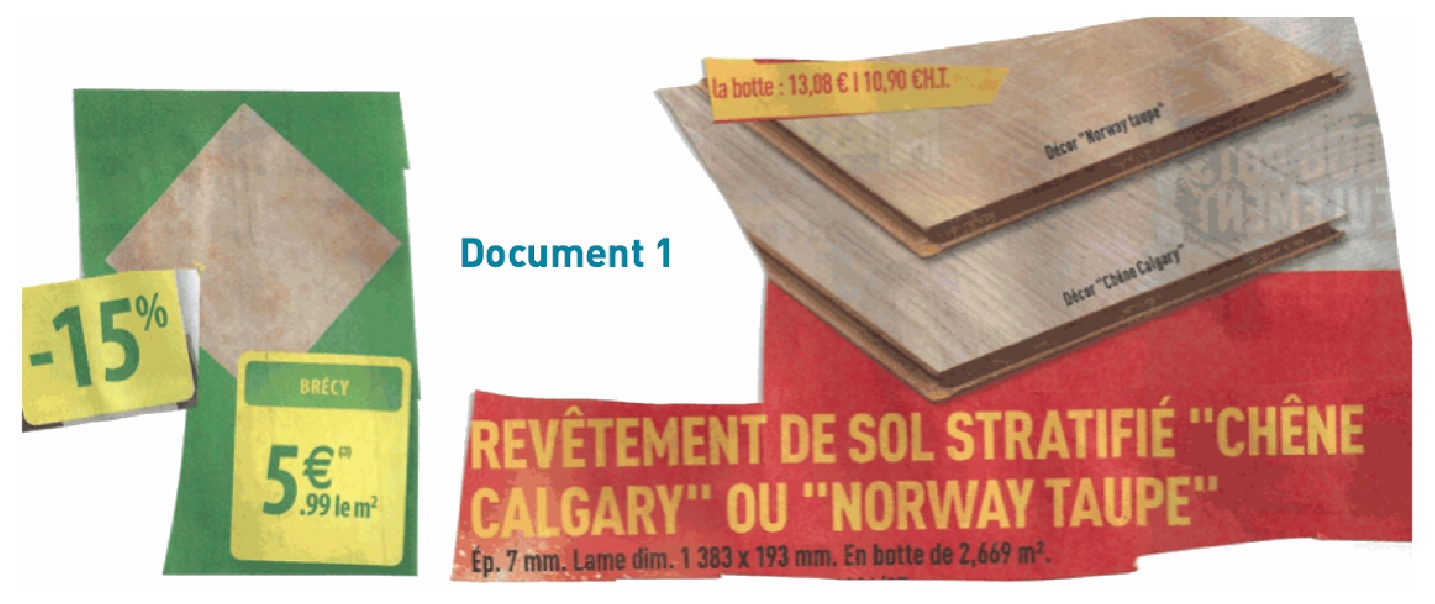
\includegraphics[width=13cm]{promotion} \\ [5mm]
      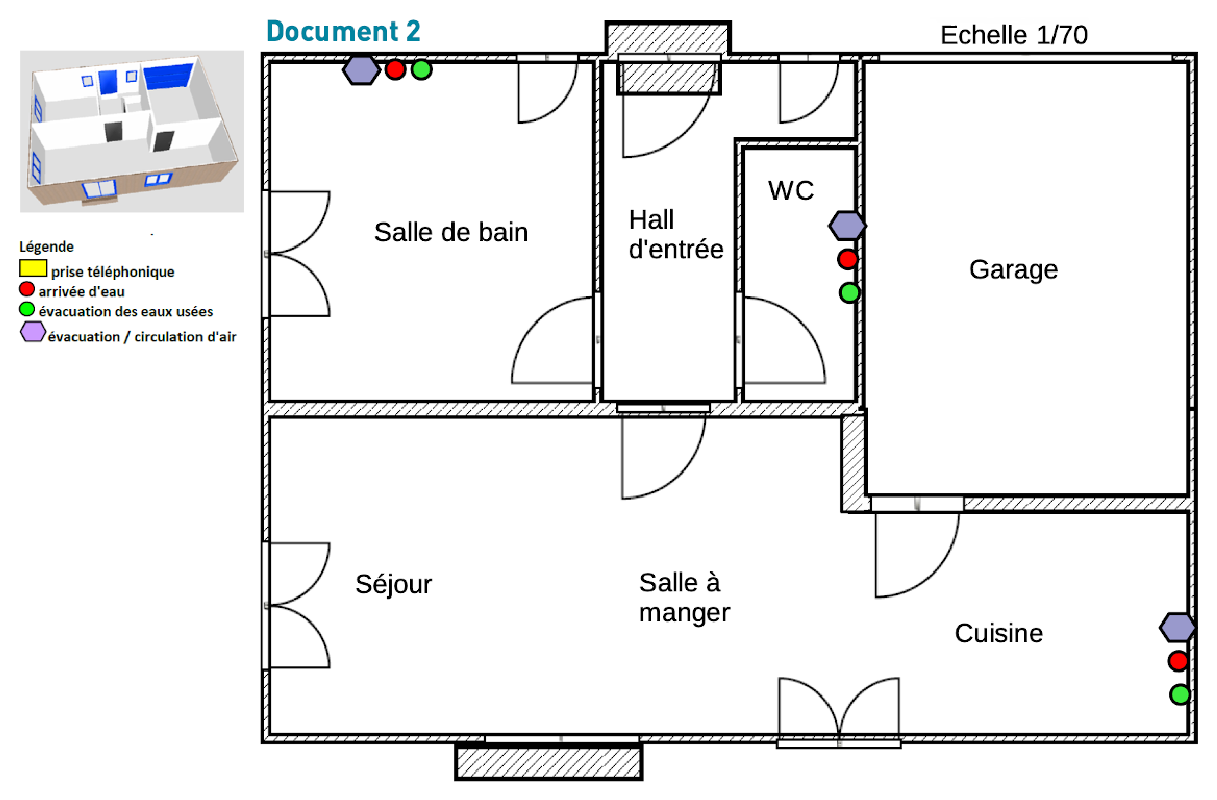
\includegraphics[width=16cm]{plan}
   \end{center}
   \partie[la tâche proposée]
    Ils veulent poser du carrelage dans la cuisine et du parquet dans le reste de la pièce. À l'aide des documents 1 et 2, aider Lucie et Marc à estimer le montant de leur facture.

\vfill\hfill {\it\footnotesize Source : éduSCOL.education.fr/ressources-2016 - résoudre des problèmes de proportionnalité.}

 
